\documentclass[../DCM2_Verslag.tex]{subfiles}
\begin{document}

Dit hoofdstuk licht de onderzoeksmethode en testopstelling toe. 

\section{ESP32}
Het platform dat onderzocht wordt is de ESP32. De ESP32 is een microcontroller van de Chinese fabrikant Espressif.\\ De microcontroller bevat een WiFi en Bluetooth (met ble) peripheral die met behulp van de open source sdk aangestuurd kan worden. De ESP32 is een veelgebruikte microcontroller in de hobbyscene. Dit komt voornamelijk door de goede ondersteuning voor de arduino sdk en de ingebouwde WiFi peripheral.
\\\\
Andere redenenen voor de populariteit van deze microcontroller zijn:\\
- De twee xTensa lx6 kernen\\
- 4 MB flash (uitbreidbaar tot 16MB met een SPI flash chip)\\
- 320Kb ram\\
- Freertos ondersteuning\\
- Cryptographische functies voor hardware acceleratie van de tcp/ip stack en beveiligingsalgorithmen\\
- Zowel in module vorm als losse chip leverbaar.\\\\
Dit onderzoek zal gebruik maken van een ESP32 development board, het ESP32 development board heeft alle randcomponenten benodigd om de chip te programmeren en voeden. \\
\newcommand{\sectionbreak}{\clearpage}
\subsection{TCP/IP stack en Programmeer platformen}
Het platform heeft verschillende soorten tcp/ip stacks en programmeer platformen. Zo zijn er programmeer platformen als: Mongoose os, Zerynth, NodeMCU en ESP-IDF met freertos.\\ Het platform wat gekozen is voor dit onderzoek is ESP-IDF met freertos. 
\\Bij dit platform zit een tcp/ip stack meegeleverd, de tcp/ip stack die is meegeleverd is een aangepaste versie van de lwIP(lightweight tcp/ip stack) tcp/ip stack. 
\\De aanpassingen zijn gedaan door de fabrikant zijn om lwIP beter te integreren in de bestaande software van de ESP-IDF SDK. 
\\Voorbeelden van modificaties die zijn aangebracht aan de lwip library zijn onder andere: \\\\
- Het thread safe maken van sockets\\
- Timers uitzetten als er geen gebruik van wordt gemaaakt of als er een timeout situatie optreed\\
- IPV4 en IPV6 multicast socket opties toevoegen\\
- Het toevoegen van aan IPV4 gekoppelde IPV6 adressen\\
- Het toevoegen van geadvanceerde configureerbare hooks aan het build systeem.\\\\
Naast dat de ESP32 een tcp/ip stack gebruikt, gebruikt de andere host waarmee de ESP32 verbindt ook een TCP/IP stack. Bij dit onderzoek is de andere host een PC met een Manjaro Linux variant. Deze host maakt gebruik van de Linux Kernel TCP/IP stack. Deze TCP/IP stack is een direct afgeleide versie van de BSD TCP/IP stack en ondersteunt ook de volledige BSD TCP/IP stack. Ook in het linux ecosysteem zijn er andere opties voor TCP/IP stack, zoals PF-RING, Snabbswitch, DPDK en Netmap. Om praktische redenen wordt er in dit onderzoek gebruik gemaakt van de standaard met linux meegeleverde Linux kernel tcp/ip stack. \\
De compiler die gebruikt wordt in dit onderzoek voor de ESP32 is de Xtensa ESP32 GCC compiler (2021r2-8.4.0). In het build systeem is er gebruik gemaakt van CMake(3.20.3) en Ninja(1.10.2).\\
De compiler die gebruikt wordt in dit onderzoek op de PC is GCC(12.2.0). In het build systeem is er gebruikt gemaakt van cmake(3.24.3) en ninja(1.11.1). Voor scripting wordt er gebruik gemaakt van Python(3.10.8).\\
\section{Testmethode}
\subsection{iperf}
Om op een industriestandaard wijze te kunnen testen wordt er gebruik gemaakt van het programma Iperf om de bandbreedte testen uit te kunnen voeren.\\
Deze manier van testen kan het hele systeem (WiFi peripheral, memory management en tcp/ip stack) testen. Bovendien heeft iperf opties om package sizes, window sizes en andere variabelen gebruikt in dit onderzoek aan te kunnen passen. Om Iperf te kunnen gebruiken op de ESP32 wordt er gebruik gemaakt van het Iperf voorbeeld geleverd door de fabrikant. Dit voorbeeld levert een vrijwel complete implementatie van Iperf v2.\\\\
Iperf werkt door een verbinding tussen twee hosts te maken met tcp of udp sockets en vervolgens pakketten met een vaste grootte over deze verbinding te sturen gedurende een bepaalde tijd. De tijd is instelbaar en is normaal 10 seconden. In deze 10 seconden houdt het programma bij hoeveel pakketten er verstuurd zijn (en goed ontvangen) en bepaald hieruit wat de bandbreedte is van de verbinding.\\
\begin{figure}[h]
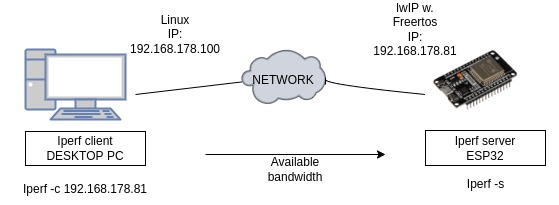
\includegraphics[scale=0.6]{Iperf_diagram_esp_as_server}
\caption{Iperfs werking met ESP32 als server}
\end{figure}
\begin{figure}[h]
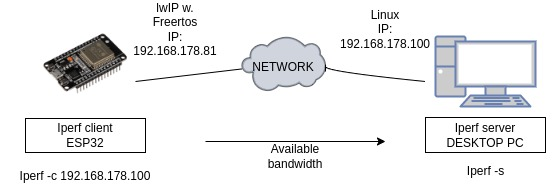
\includegraphics[scale=0.6]{Iperf_diagram_Desktop_as_server}
\caption{Iperfs werking met ESP32 als client}
\end{figure}
\subsection{Negatieve factoren}
Er zijn verschillende factoren die de performance van de tcp/ip stack negatief kunnen beïnvloeden. Voorbeelden van deze factoren zijn ruis over het medium, de snelheid van de interne communicatiebus tussen de PHY en de microcontroller, de snelheid van het geheugen en het antenne ontwerp van de WiFi controller.\\\\
Espressif, de fabrikant van de ESP32 heeft dezelfde testen uitgevoerd (als dit onderzoek) met behulp van Iperf. Waarbij de testen in zowel een open ruimte als in een afgeschermde (shielded) doos (samen met de access point) zijn uitgevoerd. Uit de resultaten zijn duidelijk af te leiden dat ruis en andere externe factoren een grote invloed hebben op de performance van de WiFi verbinding en daarmee ook de TCP/IP stack.\\
\begin{figure}[h]
\begin{tabular}{||l|c|r|p{6cm}||}
	 \hline
 	 Type & Air in lab & Shielded box & Test tool \\
  	 \hline \hline    
   	 UDP RX & 30 MBit/s & 85 MBit/s & iperf example \\
   	 UDP TX & 30 MBit/s & 75 MBit/s & iperf example \\
   	 TCP RX & 20 MBit/s & 65 MBit/s & iperf example \\
   	 TCP TX & 20 MBit/s & 75 MBit/s & iperf example \\
\end{tabular}
\caption{ESP32 Wi-Fi Throughput volgens Espressif}
\end{figure}
\\Dit onderzoek zal zich alleen richten op open lucht testen of zoals in het tabel hierboven benoemd Air in lab. Met de Wi-Fi access point naast de ESP32 en de PC bekabeld verbonden met de Wi-Fi accesspoint. Om de externe invloeden zoals ruis te beperken.

\subsection{Testopstelling}
Om het onderzoek repetitief onder dezelfde condities uit te kunnen voeren is er een testopstelling gemaakt. Deze testopstelling bestaat uit een ESP32, een Wi-Fi router en een Desktop PC met een variant van linux. De desktop pc is bedraad verbonden met de Wi-Fi router en de ESP32 is draadloos verbonden. De Wi-Fi router die gebruikt wordt is een Fritzbox 7390, dit modem heeft een theoretische maximale bandbreedte van 300Mbps (Wireless N), dit is voldoende voor de ESP32 die een theoretisch haalbare bandbreedte heeft van 54Mbps (Wireless G). Hieronder is de testopstelling geillustreerd in een diagram:
\begin{figure}[h]
\centering
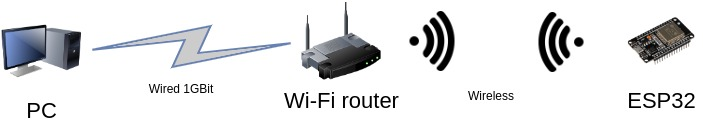
\includegraphics[scale=0.4]{Network_topology_test}
\caption{Testopstelling schematisch uitgedrukt}
\end{figure}

\subsection{Uitvoering}
Het onderzoek wordt uitgevoerd door een script die automatisch de bandbreedte testen uitvoerd. Het script test ook de package sizes en window sizes. Dit doet het script door een nulmeting te doen met de standaard opties van Iperf. Vervolgens gaat het script de window size of package size aanpassen en vergelijken met de nulmeting. Het script verzamelt de gegevens en geeft een tabel wat meegenomen kan worden in dit rapport.

\subsection{Testscript}
Om de resultaten van het onderzoek te verzamelen is er een testscript geschreven in python. Dit script zal 3 testrondes uitvoeren en vervolgens een gemiddelde trekken uit de verzamelde gegevens.
Deze gegevens zal het script netjes in een tabel zetten zodat het overgenomen kan worden in dit verslag. Het script wordt uiteraard aan het einde van het verslag in het hoofdstuk bijlagen erbij gezet.
\end{document}
